\documentclass[12pt]{article}
\usepackage[utf8x]{inputenc}
\usepackage{tgcursor}
\usepackage[serbian]{babel}
\usepackage{geometry}
\usepackage{subcaption}
\usepackage [export]{adjust box}
\usepackage{tcolorbox}
\geometry{a4paper} 
<<<<<<< HEAD
\renewcommand{\contentsname}{Sadržaj}
\usepackage{indentfirst}
\usepackage {listings}
\usepackage{hyperref}
\usepackage{color}

\definecolor{codegreen}{rgb}{0,0.6,0}
\definecolor{codegray}{rgb}{0.5,0.5,0.5}
\definecolor{codepurple}{rgb}{0.58,0,0.82}
\definecolor{backcolour}{rgb}{0.95,0.95,0.92}

\lstdefinestyle{mystyle}{
	backgroundcolor=\color{backcolour},   
	commentstyle=\color{codegreen},
	keywordstyle=\color{magenta},
	numberstyle=\tiny\color{codegray},
	stringstyle=\color{codepurple},
	basicstyle=\footnotesize,
	breakatwhitespace=false,         
	breaklines=true,                 
	captionpos=b,                    
	keepspaces=true,                 
	%numbers=left,                    
	numbersep=5pt,                  
	showspaces=false,                
	showstringspaces=false,
	showtabs=false,                  
	tabsize=2
}

\lstset{style=mystyle}






=======

\renewcommand{\contentsname}{Sadržaj}
\usepackage{indentfirst}
\usepackage {listings}

\usepackage{hyperref}
>>>>>>> origin
\begin{document}
\pagenumbering{gobble}
\clearpage

\begin{figure}[h]

\includegraphics[width=0.3\linewidth]{PMF.jpg}

\includegraphics[width=0.3\linewidth,right=10cm]{uns.jpg}
\end{figure}

\begin{center}
{\Large Univerzitet u Novom Sadu\\\Large Prirodno - matematički fakultet,\\ \Large Departman za fiziku}
\end {center}
\begin{center}
\vspace{3.cm}
{\Large  \textbf{UPOTREBA PROGRAMSKI JEZIK PYTHON U ANALIZI METEOROLOŠKIH PODATAKA}}
\end {center}
\vspace{1.cm}
\begin{center}
\Large -MASTER RAD-
\end{center}
\vspace{3cm}
\begin{center}Mentor: Prof.dr Ilija Arsenić\hfill Kandidat: Martin Petraš
\end{center}
\vspace{0.5cm}
\begin{center}
Novi Sad, 2018.
\end{center}
\newpage
\pagebreak
\begin{center}
\tableofcontents
\end{center}
\newpage
\pagebreak
\pagenumbering{arabic}

\newpage
\section*{\textsl{Zahvalnica:}}
\textsl{mami,tati,..............................}
\newpage
\begin{center}
\section*{Uvod}
\end{center}
Predmet ovog rada je izrada web aplikacije u Django razvojnom okruženju za analizu srednje temperature na visini od dva metra od površine tla. Web aplikacija koristi podatke iz \textit{Carpatoclim} projekta, projekat koji se bavio prikupljanjem meteoroloških podataka u vremenskom periodu od 1961-2010 godine. Obuhvaćena oblast, kao što i samo ime projekta kaže, je oblast  pružanja planinskog lanca Karpatskih planina. Aplikacija će korisniku omogućiti prikaz podataka u vizuelnom grafičkom obliku za navedeni vremenski interval. Kako bi ubrzali proces grafičkog crtanja, podatke o srednjoj temperaturi smo upakovali u SQLite data bazu, koja je podrazumevana data baza za Django programski okvir\footnote{Programski okvir ili na engleskom framework predstavlja univerzalano softversko okruženje koje može biti korišćeno iznova i koje omogućava određenu funkcionalnost kao deo veće softverske platforme da olakša razvoj aplikacija, proizvoda i rešenja}. Aplikacija omogućava informativni prikaz za zadate kordinate tačke, u kojoj državi odnosno altitudi se nalazi. 
Rad će biti podeljen na četiri dela. Prvi deo se bavi kratkim opisom korišćenih paketa. Drugi deo se bavi postupkom instaliranja i podešavanja okruženja, konfigurisanjem Django projekta. Treći deo opisuje primenjen metod interpolacije dok se četvrti deo bavi samom aplikacijom. 
\newpage

\section{Korišćeni alati}

\subsection{Python} 

Python je dinamički i objektno orijentisan programski jezik. Spada u interpreterske programske jezike visokog nivoa. Nastao je krajem devedsetih godina prošlog veka i njegov autor je Gvido van Rosum.  Broj funkcija u samom jeziku je skroman, pa zahteva relativno malo uloženog vremena i napora kako bi se napravio prvi programi. Pythonova sintaksa je dizajnirana da bude čitljiva i jednostavna, što ga čini idealnim nastavnim jezikom i omogućava početnicima brzo napredovanje. Programeri provode više vremena razmišljajući o problemu koji pokušavaju da reše, a manje vremena razmišljaju o kompleksnosti jezika. Python se može izvoditi na svim važnijim operativnim sistemima (Windows, Linux, OS X). Za pokretanje Python programa potreban je Python interpreter, koji je pisan u programskom jeziku C. 
Najosnovnije korišćenje Pythona je kao jezik skriptovanja i automatizacije, koristi se za nauku o podacima i mašinsko učenje, za web usluge, metaprogramiranje. Njegova popularnost, sem čiste i pregledne sintakse, ogleda se i u velikom broju standardnih biblioteka koje su najčešće pisane u C i samom Pythonu jeziku. Kao nedostatak ovog programskog jezika istakli bi njegovu brzinu, međutim brzina kojom se može napisati funkcionalan program je daleko brži nego u nekom drugom jeziku.  


\subsubsection{Korišćenje biblioteka}
Mnoge Python funkcije su sadržane u specijalizovanim bibliotekama, tzv. modulima. Učitavanje modula se postiže naredbom \textsl{import}. Python je prvo svoju popularnost stekao pri izradi web aplikacija, međutim usavršavanjem podrške za dodtane module otvorilo je vrata Pythonu i u drugim oblastima programiranja. Moduli poput \textsl{numpy} i \textsl{pandas}, koji se koriste za analizu i vizuelno obradu podataka, su Python svrstali uz rame sa ostalim kako komercijalnim programima tako i sa programima otvorenog koda kao što su R, MATLAB, SAS, Stata. Kada uzmemo u obzir da Python spada u besplatni programski jezik, njegova popularnost nije slučajnost. Jedan deo ove popularnosti u obradi podataka pripada i laka integracija sa C, C++ i FORTRAN kodom.  
Mogućnosti koje pružaju biblioteke je moguće izvesti koristeći isključivo samo Pythonov kod. Prednost biblioteka je u efikasnosti i lakoći kojim se postižu isti rezultati, uz manje utrošenog vremena. Jedna od značajnih biblioteka otvorenog koda je i SciKit. Ona sadrži različite klase objekata za kasifikaciju, algoritme mašinskog učenja (engl. \textsl{Machine Learning}). U SciKit paketu se nalaze  NumPy i SciPy biblioteke koje sadrže klase za razne standardne matematičke i numeričke funkcije. 
\subsubsection{Scipy}
Scipy (engl. \textsl{Scientific Python}) proširuje funkcionalnost Numpy-a sa značajnom zbirkom algoritama za Fourijeovu transformaciju, regresiju i druge matematičke tehnike. Pored modula za interpolaciju, koji je nama značajan, sadrži još neke module poput :
\begin{itemize}
\item scipy.integrate - integraciija funkcija
\item scipy.special - specijalne funkcije
\item scipy.optimize - optimizacija
\end{itemize}

\subsubsection{Numpy}
Numpy (\textsl{Numerical Python}) predstavlja fundamentalnu open source Python biblioteku kada se u obzir uzmu numerički proračuni. Sadrži matematičke funkcije zadužene za operaciju na podacima, koje se veoma brzo i efikasno izvršavaju. Poziva se komandom : 
\begin{lstlisting}
 import numpy as np
\end{lstlisting}
Za numeričke proračune, formirani nizovi korišćenjem Numpy su dosta efikasniji prilikom njihove manipulacije nego bilo koja druga izgrađena struktura unutar Pythona. Biblioteka je pisana u C-u i Fortranu. 
\subsubsection{Pandas}
Pandas je dizajniran kako bi se ubrzao rad sa strukturiranim ili tabelarnim podacima i kao takav, postala jako moćna i produktivna alatka za analizu podataka. Ono što krasi ovu biblioteku je i velika podrška od strane zajednice, njen aktivan razvoj, odličan rad sa ostalim bibliotekama. Neke od mogućnosti koje pruža ova biblioteka su:
\begin{itemize}
  \item ulaz-izlaz podataka u različitim formatima (csv, txt, SQL...)
  \item indeksiranje, sortiranje, rangiranje
  \item filtriranje podataka 
  \item grupisanje
  \item vizuelizacija
\end{itemize}
Sačinjenja je od dve strukture podataka, \textsl{dataframe} i \textsl{series}. \textsl{Series} predstavljaju jednodimenzioni objekat sačinjen od tabele sa vrednostima i njihovim indeksima, dok \textsl{dataframe} takođe predstavlja tabelarnu strukturu definisanu u dve ili više dimenzija. Najčešće korišćenja skraćenjica za \textsl{pandas} je \textsl{pd}, poziva se korišćenjem komande :
\begin{lstlisting}
 import pandas as pd 
\end{lstlisting}
Za čitanje baze podataka korišćena je komanda :
\begin{lstlisting}
 pd.read_sql_query
\end{lstlisting}
\subsubsection{Matplotlib}
Ova biblioteka se koristi za vizuelizaciju podataka. U kombinaciji sa \textsl{numpy} i \textsl{pandas} čine jako moćne alate, koji se mogu nositi sa komercijalnim i dosta skupljim alatima kao što su \textsl{Matlab} i \textsl{Mathematica}. Mana ove biblioteke je potreba za pisanjem većeg broja linija koda radi dobijanja naprednije vizuelizacije. 
Povećanjem potrebe za kvalitetnijom vizuelizacijom, nastale su biblioteke, koje se u većoj ili manjoj meri oslanjaju na \textsl{matplotlib}. Jedna od takvih biblioteka je \textsl{seaborn}, čiji je fokus na atraktivnijoj izradi statističkih grafika. \textsl{Seaborn} se potpuno oslanja na \textsl{matplotlib}. Naveo bih još i \textsl{bokeh} i \textsl{altair} koje nisu zavisne od \textsl{matplotlib}, a takođe se koriste za vizuelizaciju podataka.
\subsubsection{Metpy}
Metpy predstavlja kolekciju alata koje dopunjuju Python module i koriste se za pregled, vizuilizaciju i proračune meteoroloških podataka. Paket je nastao od strane \textsl{Unidata} udruženja, koja se bavi izradom softverskih alata u naučne svrhe. Za instaliranje Metpy alata, u terminal kucamo sledeću komandu :
\begin{lstlisting}
 pip install metpy
\end{lstlisting}
Prilikom interpolacije polja temperature korišćena je funkcija\textit{ metpy.interpolate}, koja je se bazira na \textit{scpy.interpolate} funkciji, razlika je u brzini interpolacije. 

\newpage

\subsection{Django}

Nagla ekspanzija interneta praćenja je i povećanjem popularnosti web aplikacija. Google, Facebook, YouTube su samo od nekih popularnih web aplikacija koje čine svakodnevnicu pretraživanja. Web aplikacija je u stvari program, kojim pristupamo pomoću internet pretraživača (browser). Ovakav pristup omogućava veću bezbednost, sigurnost bez potrebe za instaliranjem na operativni sistem. Sve što je potrebno jeste uređaj koji ima pristup internetu. 
Usled spomenutog naglog rasta popularnosti web aplikacija, javila se potreba za brzim i automatizovanim načinom njihove izrade. Tako je nastao Django, web framework napisan u Pythonu koji služi za izradu web stranica i aplikacija. 

Razvijan je od 2003. godine od strane novinara, koji su zahtevali brzo razvojno okruženje za izradu web stranica. Kao slobodni softver (eng. \textsl{open source}) objavljen je 2005. godine, kada je i dobio ime Django po jazz gitaristi Djangu Reinhardtu. Od 2008. godine za razvoj Django frameworka zadužena je \textsl{Django Software Foundation}.
Django je zapravo skup alata i biblioteka koje programerima web aplikacija olakšavaju rad. Dizajniran je kako bi se skratilo vreme potrebno za izradu web aplikacije, držeći se strogih zahteva iskusnih web programera koji su ga stvorili. Web programiranje zahteva ponavljanje isti zadataka kao što su :
\begin{itemize}
\item korisnička prava
\item registracija korisnika
\item konfigurisanje URL-ova
\item validacija unesenih podataka
\item administracija sajta
\end{itemize}
 
\subsubsection{Django arhitektura}
Kao što je rečeno, Django služi za brzu i jednostavnu izradu web stranica i aplikacija. Ovu osobinu mu omogućava arhitektura MVC (\textsl{model-view-controller}) na kojoj se bazira, i koja razdvaja logiku same aplikacije od prikazanog dela aplikacije. Možemo je podeliti na tri dela:
\begin{itemize}
\item Model 
\item View (Pogled)
\item Controller(Kontroler)
\end{itemize}
\begin{figure}[h!]
\centering
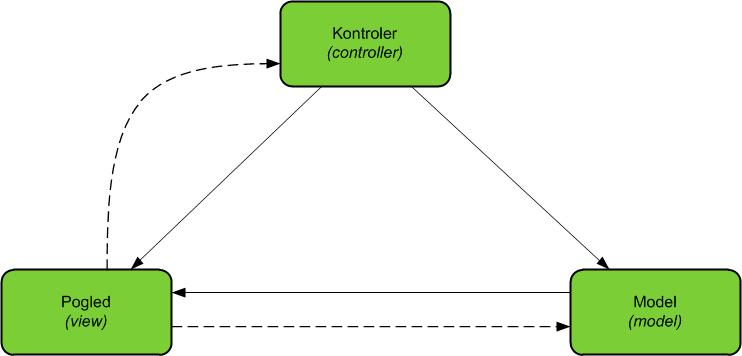
\includegraphics[width=0.6\linewidth]{django.jpeg}
\caption*{\textsl{Slika 1. Koncept modela MVC }}
\end{figure}
Pune linije predstavljaju vezu izmedju navedenih elemenata za razmenu podataka, dok isprekidane linije predstavljaju vezu kod koje neki drugi objekt vrši tu funkciju. Django koristi drugačije nazive elemenata modela MVC. Tako \textsl{view} predstavlja kontroler a \textsl{template} (šablon) predstavlja \textsl{view} iz MVC modela. Implementaciju MVC modela kod Django frameworka možem nazvati MTV (\textsl{model-template-view}). Ova promena je objašnjena na takav način, što se kod Djanga pogledom predstavljaju podaci koji se prezentuju, dok šablon predstavlja način na koji se podaci prikazuju. 

Model je zadužen za komunikaciju, odnosno opis baze podataka sa kojom je Django povezan. Model je u Django okruženju klasa (engl. \textsl{class}) i određuje varijable i metode pridružene određenim tipovima podataka. Pridružene varijable predstavljaju kolone u tablici dok metode definišu relacije između varijabli.  Ulog modela je da dohvati tražene podatke i prosledi ih ka pogledu. Model nema informacija o šablonima i funkcijama izvedenih u pogledima. 

Uloga pogleda je prikazivanje podataka dohvaćenih iz baze podataka u internet pretraživaču. Priliko izrade web stranice, svaka kreirana aplikacija ima svoj pogled.  Pogled u stvari sačinjavaju funckije u Pytho programskom jeziku.  Ove funkcije imaju ulogu prenosnika podataka koji će biti prikazani.  

Pregled je HTML stranica s dodatnim strukturama koje omogućavaju prikaz podataka koji su poslati od pogleda.  Uloga pregleda je da sadržaj poslat od strane pogleda ugradi u HTML kod, koji će se prikazati u internet pretraživaču. 

\newpage
\section{Postupak za instaliranje}
\subsection{Instaliranje Python3 verzije }
Django je pisan u Python-u i kako bi ga koristili potrebno je imati instaliran Python. Python kao programski jezik postoji za sve tri popularne sistemske platforme Windows, Linux i OSX. Ovde će biti prikazan postupak instaliranja potrebnih paketa za rad pod Linux operativnim sistemom. Gotov sve distibucije linuxa dolaze sa instaliranim Python-om, razlika može biti u verziji. Postoje dve verzije, starija 2.7 verzija koja je podržana do kraja 2020. godine, i novija verzija 3.6. U radu je korišćena verzija 3.5. Proveru verzije radimo tako što otvorimo terminal i kucamo sledeću komandu : 
\begin{lstlisting}
 python3 --version
\end{lstlisting}
Ukoliko je Python verzije 3.6 instaliran, pojavi se sledeće
\begin{lstlisting}
 Python 3.6.6
\end{lstlisting}
\begin{figure}[h!]
\centering
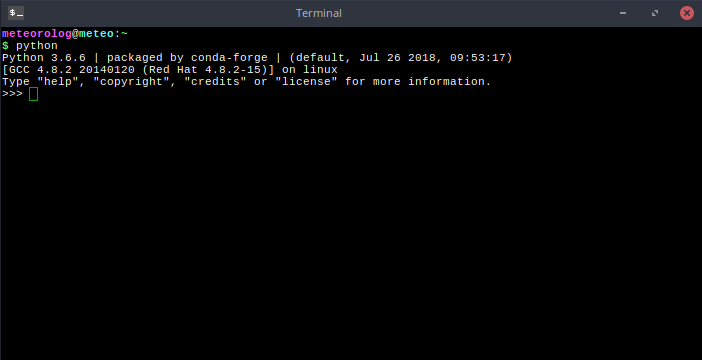
\includegraphics[width=0.8\linewidth]{python.png}
\caption*{\textsl{Slika 2. Python verzije 3.6 pokrenut iz terminala}}
\end{figure}
Ukoliko nemate instaliran Python verzije 3.6, možete ga instalirati :
\begin{lstlisting}[language=Python]
 sudo apt install python3.6 
\end{lstlisting}

\subsection{Podešavanje virtuelnog okruženja}
Pre nego što instaliramo Django pokazaćemo kako instalirati veoma zahvalnu alatku, koja nam omogućava održavanje čistoće paketa na sistemu. Virtuelno okruženje (engl. \textsl{virtual environment}) izoluje projekte jedan od drugog, držeći pakete vezane za svaki projekat zasebno. Kako bi kreirali virtuelno okruženje zvano \textsl{env}, u direktorijum u kome smo započeli projekat, u terminal kucamo :
\begin{lstlisting}
 python3 -m virtualenv env
\end{lstlisting} 
Kada ovo odradimo, u dokumentu se pojavi dokument \textsl{env} u koji će se instalirati svi paketi koje u buduće budemo koristili. Kada ovo sve odradimo, ostalo nam je još da ovo virtuelno okruženje aktiviramo. Aktiviranje virtuelno okruženja radimo na sledeći način :
\begin{lstlisting}
 source env/bin/activate
\end{lstlisting} 
nako čega se u terminalu pojavljuje nastavak \textsl{(env)}. Ovaj nastavak nam potvrđuje da je virtuelno okruženje aktvirano. Kako bi zatvorili virtuelno okruženje, u terminal kucamo komandu \textsl{deactivate}. 
\begin{figure}[h!]
\centering
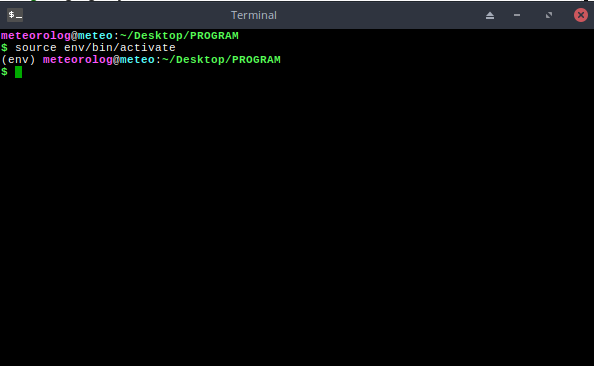
\includegraphics[width=0.8\linewidth]{env.png}
\caption*{\textsl{Slika 3. Postupak aktiviranje virtuelnog okruženja}}
\end{figure}

\subsection{Pokretanje Django projekta}
<<<<<<< HEAD
Kada smo podesili virtuelno okruženje možemo instalirati Django.  Instaliranje radimo pomoću \textsl{pip} menadžera. Prvo uradimo nadogradnju pip paketa, kako bi imali poslednju verziju. To radimo na sledeći način :
=======
Kada smo podesili virtuelno okruženje možemo instalirati Django.  Instaliranje radimo pomoću  \textsl{pip} menadžera-. Prvo uradimo nadogradnju pip paketa, kako bi imali poslednju verziju. To radimo na sledeći način :
>>>>>>> origin
\begin{lstlisting}
python3 -m pip install --upgrade pip
\end{lstlisting} 
Kada smo uradili nadogradnju pip-a, Django instaliramo :
\begin{lstlisting}
pip install django
\end{lstlisting}
Kada ovo odradimo možemo uspešno pokrenuti naš prvi Django projekat. Izrada projekta podrazumeva pokretanje Django skripte koja će izgraditi kostur potrebnih dadoteka. Kucamo sledeću komandu :
\begin{lstlisting}
django-admin startproject carpatclimsite .
\end{lstlisting} 
<<<<<<< HEAD
i u stvorenom direktorijum dobijamo strukturu kao sa slike 4. U strukturi django projekta \textsl{manage.py} skripta predstavlja upravitelja projekta pomoću kojeg se pokreće web server. Skripta        \textsl{settings.py} služi za konfigurisanje našeg sajta. \textsl{urls.py} sadrži šablone (preglede) koje koristimo. Kako bi pokrenuli web server u terminal kucamo : 
\begin{lstlisting}{centering}
python manage.py runserver
\end{lstlisting}nako čega u internet pretraživač unesemo adresu $http://127.0.0.1:8000/$.  Ako je sve urađeno kako treba u internet pretraživaču bi trebalo da se pojavi čestitka o uspešnom pokretanju web sajta.
\begin{figure}[h!]
	\centering
	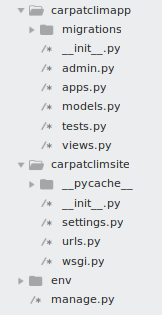
\includegraphics[width=0.33\linewidth]{Kosturapp.png}
	\caption*{\textsl{Slika 4. Struktura carpatclimsite projekta}}
\end{figure}
Nakon uspešnog pokretanja sajta, sledeća stavka je stvaranje aplikacije. Kako bi stvorili aplikaciju u datom projektu, u terminal upisujemo sledeću komandu :
\begin{lstlisting}{centering}
python manage.py startapp carpatclimapp
\end{lstlisting}
Nakon ove komande u projektu se pojavi dokument carpatclimapp sa Python skriptama. U Python skripti \textit{views.py} (pogled) skripta sadrži funkcije zadužene za funkcionisanje web aplikacije. Pomoću pogleda definišemo kontak sa bazom podataka, vršimo razmenu podataka. Svaki pogled se mora definisati u \textsl{urls.py} skripti koju stvorimo u ovom dokumentu. Sledeća bitna skripta je forms.py, pomoću koje vršimo definisanje godine, meseca, dana za pruzimanje podataka iz baze podataka. Ovu skriptu kao i \textsl{urls.py} moramo stvoriti u carpatclimapp dokumentu. U \textsl{forms.py} skripti definišemo klase za :
\begin{itemize}
	\item Godišenje (CronFormYearly)
	\item Mesečne (CronFormMonthly)
	\item Dnevne (CronFormDaily)
\end{itemize}
vrednosti srednjih temperatura. U zavisnosti od izbora željenog vremenskog intervala, pojavi se odgovarajuća forma.
\subsubsection{POST i GET zahtev}
Kako bi što bolje razumeli interakciju između forme i pogleda, njihovo funkcionalnost ćemo objasniti uz pomoć POST i GET zahteva. Koristeći formu stvaramo podatke koje uz pomoć POST metoda šaljemo ka serveru u vidu zahteva (\textsl{Request}), nakon čega server vraća zahtevane podatke u vidu odgovora (\textsl{Response}). Forma stvara zahtev koje podatke želimo primiti kada se stisne dugme "{Submitt}". GET metoda se koristi za dostavljanje podataka u niz i stvaranje URL adrese. 
\begin{figure}[h!]
	\centering
	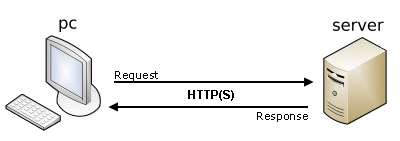
\includegraphics[width=0.6\linewidth]{server.png}
	\caption*{\textsl{Slika 5. Razmena podataka između korisnika i servera}}
\end{figure}
Uloga pogleda je ostvarivanje kontakta sa serverom i stvaranje prikaza podataka kada oni stignu sa servera. Prikaz se ostvaruje uz pomoć  šablona  (templates), koje se moraju stvoriti u dokumentu date aplikacije. Za svaku aplikaciju unutar Django projekta se stvaraju zasebni šabloni čija uloga je vizuelni u sklopu internet pretraživača. U te svrhe pored HTML i CSS korišćen je i Bootstrap.

Pogledaćemo sada kako izgleda pogled za godišnje vrednosti temperature.
\begin{lstlisting}[language=Python]
def yearly(request):
	if request.method == "POST":
		form = CronFormYearly(request.POST)
		if form.is_valid():
			data = form.cleaned_data
			year = data.get('year')
			date_path = year
			return redirect('/%s/' % (date_path))
	else:
		form = CronFormYearly()
		active_yearly = True
	return render(request, 'carpatclimapp/home.html', {'form': form, 'active_yearly': active_yearly})
\end{lstlisting} 
Ovaj pogled, koji definiše upit za godišnje podatke, nam kaže sledeće, ako je aktiviran POST metod, uzmi formu u obliku \textsl{CronFormYearly}, ako je forma važeća uzmi podatke za definisanu godinu. Ako POST zahtev nije aktiviran, prikaži formu čija struktura je definisana u $home.html$ datoteci, koja je deo bloka \textsl{base.html}.

\subsubsection{Grafički prikaz polja temperature}
Kada smo poslali zahtev za podatake, i kada su ovi podaci uspešno prosleđeni, sa njima želim nešto dobiti. U našem slučaju mi želimo dobiti grafički prikaz polja srednje temperature u sklopu Karpata za zadatu godinu. Kako bi dobili grafički prikaz moramo stvoriti funkciju koja će ovaj zadatak uraditi za nas. U te svrhe je zadužena funkcija \verb|carpatclim_y_figure|.
\begin{lstlisting}[language=Python]
def carpatclim_y_figure(request, year):

map = create_map(year, month=None, day=None)
buffer = BytesIO()
canvas = FigureCanvas(map)
canvas.print_png(buffer)

response = HttpResponse(buffer.getvalue(), content_type='image/png')
response['Content-Length'] = str(len(response.content))
return response
\end{lstlisting}
Uzimajući vrednosti za godinu, koristeći funkciju \verb|create_map| dobija se grafički prikaz polja temperature.

\subsubsection{Definisanje URL-a}
Kako bi pokrenuli funkciju \verb|yeraly| i \verb|carpatclim_y_figure|, koje se nalaze u sklopu pogleda, moramo definisati njihov url. To se radi tako što unutar carpatoclimapp stvorimo skriptu \textsl{urls.py}, unutra koje definišemo urlpatterns za funkcije:
\begin{lstlisting}[language=Python]
path('yearly/', views.yearly, name='yearly'),
path('<int:year>/figure.png', views.carpatclim_y_figure, name='carpatclim_y_figure')
\end{lstlisting}
Ovim pristup postižemo da za svaku funkciju postoji zadata adresa. Recimo, korišćenjem \verb|yearly/| u adresi prikazuje se forma u obliku kao na slici 6 :


\begin{figure}[h!]
	\centering
	
\includegraphics[width=0.25\linewidth]{Yearly.png}
	\caption*{\textsl{Slika 6. Izgled forme za godinšnje vrednosti}}
\end{figure}
U ovom primeru je prikazan url za godišnje vrednosti. Za mesečne i dnevne vrednosti adrese se razlikuju po tome što se osim godine, u adresi pojavljuju vrednosti za mesec odnosno dan.
%definisemo url.py, templates
%susection o kreiranju baze podataka
=======
i u stvorenom direktorijum dobijamo strukturu kao sa slike 4. U strukturi django projekta \textsl{manage.py} skripta predstavlja upravitelja projekta pomoću kojeg se pokreće web server. Skripta        \textsl{settings.py} služi za konfigurisanje našeg sajta. \textsl{urls.py} sadrži šablone (preglede) koje koristimo.
\begin{figure}[h!]
\centering
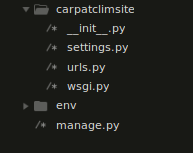
\includegraphics[width=0.5\linewidth]{kostur.png}
\caption*{\textsl{Slika 4. Izgled struktura carpatclimsite projekta}}
\end{figure}
Kako bi pokrenuli web server u terminal kucamo : 
\begin{lstlisting}{centering}
python manage.py runserver
\end{lstlisting}nako čega u internet pretraživač unesemo adresu $http://127.0.0.1:8000/$.  Ako je sve urađeno kako treba u internet pretraživaču bi trebalo da se pojavi čestitka o uspešnom pokretanju web sajta.
Nakon uspešnog pokretanja sajta, sledeća stavka je kreiranje aplikacije. Kako bi stvorili aplikaciju u datom projektu, u terminal upisujemo sledeću komandu :
\begin{lstlisting}{centering}
python manage.py startapp carpatclimapp
\end{lstlisting}Nakon ove komande u projektu se pojavi dokument carpatclimapp, sa strukturom podataka ka na slici 5. \textit{Views.py } skripta sadrži funkcije koje komunicira blblablalbl. \textsl{Modle.py} definišemo model
\begin{figure}[h!]
	\centering
	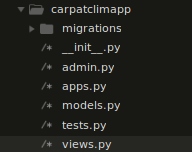
\includegraphics[width=0.5\textwidth]{app.png}
	\caption*{\textsl{Slika 5. Struktura carpatclimapp dokumenta}}
\end{figure}



  
>>>>>>> origin

\newpage
\section{Interpolacija}

Podaci sa meteoroloških stanica su veoma značajni za prognozu vremena. U prognozi vremena ovi podaci se koriste kao početni uslovi za jednačine dok se kod analize koriste za vizuelni prezentaciju polja promenljivih. Cilj je što vernije predstaviti stanje varijabli na određenom nivou i mestu. Ako bi postojala merenja u svim tačkama prostora i uz to dovoljno tačna, problem tačnosti ne bi postojao. Međutim, broj raspoloživih stanica koje šalju podatke i dalje nije dovoljan jer na nekim mestima, poput okeana ili neprisupačnim predela, ne postoji mogućnost postavljana mernih uređaja. Jedan način rešenje ovog problema su satelitska merenja a drugi pristupačniji je uz pomoć interpolacije.
\subsection{Korišćene metode interpolacije}
Interpolacija predstavlja metod procene vrednosti varijable na mestima gde oni nisu određenje, koristeći poznate vrednosti iz lokalnih lokacija. Interpolacija je moćna metoda za analizu podataka kod kojih su merenja rasuta. Problem interpolacije je njena implementacija. Za nekoliko poznatih priemera, koristeći različite metode interpolacije dobićemo različite rezultate. Zbog toga, aplikacija će omogućivati prikaz četiri metoda iterpolacije :
\begin{itemize}
\item Linearna interpolacija
\item Interpolacija najbližeg suseda
\item Barnes interpolacija
\item Cressman interpolacija
\end{itemize}
Metode interpolacije možemo podeliti u dve kategorije u zavisnosti koje tačke su uzete za definisanje interpolacije u određenoj tački. Ove dve kategorije su globalna i lokalna interpolacija.
\subsubsection{Linearna interpolacija}
U pitanju je najednostavnija i najmanje zahtevna metoda interpolacije. Interpolant se dobija uzimajući dve najbliže tačke, recimo na pozicijama $(x_{1},y_{1})$ i $(x_{2},y_{2})$ na sledeći način : 
\begin{equation}\label{key}
y= y_{1}+ \frac{(x-x_{1})(y_{2}-y_{1})}{(x_{2}-x_{1})}
\end{equation}
Mana ove metode je njena preciznost. Greška raste proporcijalno kvadratu udaljenosti između tačaka.
\subsubsection{Natural neighbor interpolacija}
Postoje razne implementacije natural neighbor interpolacija. Ovde će biti obrađena lokalna metoda koja se bazira na Voronojevom dijagramu i Deloneovoj trijangulaciji. Pokazala se kao vremenski malo zahtevna metoda, jer se bazira na ideji ponovnog korišćenja rezultata tokom proračuna u što većom obimu. Prvo ćemo definisati teoriju Voronoj dijagrama i Delonove trijangulacije.
Za dati skup tačaka u ravni, koje ćemo u daljem tekstu nazvati centrima, konstrukcija Voronoj dijagrama podrazumeva podelu ravni na ćelije, tako da svaka ćelija sadrži jedan centar. Deloneov graf nad datim skupom tačaka u ravni je dualan graf Voronoj dijagramu. Drugim rečima, čvorovi ovog grafa su centri, a grane povezuju čvorove, koji odgovaraju centrima susednih Voronoj ćelija. Na slici 5 su prikazani
Voronoj dijagram (podebljane linije) i Deloneova triangulacija (obične linije) skupa od devet centara.
\begin{figure}[h!]
	\centering
	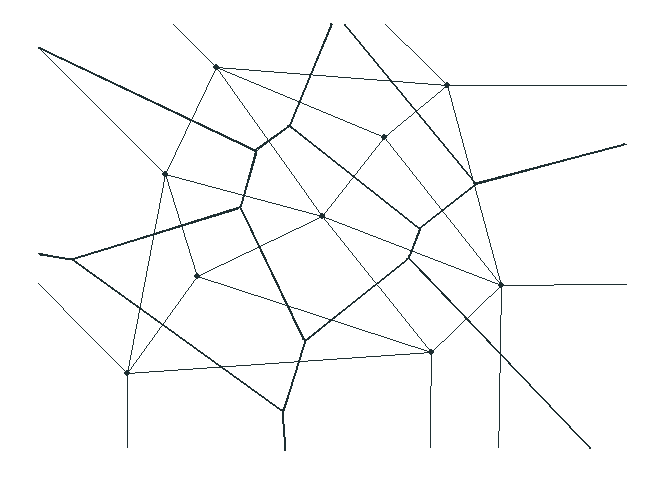
\includegraphics[width=0.5\linewidth]{vor.png}
	\caption*{\textsl{Slika 5. Voronoj dijagram i Deloneova tiangulacija}}
\end{figure} 
Ako dve Voronoj ćelije dele zajedničke ivice onda za njih kažemo da su prirodni susedi(natural neighbor). Kako bi se definisali susedi za određene tačke interpolacije $x$, prvo formiramo Voronoj ćeliju u kojoj se ova tačka nalazi. Formiranjem ćelije definišemo zapreminu $V(x)$, koja će imati nove susede. Na slici 6 možemo videti da su za tačku $x$ prirodni susedi $x_{1}$, $x_{2}$, $x_{3}$, $x_{4}$, $x_{5}$, odnosno da Voronoj ćelija $V(x)$ deli ivice sa $V(x_1)$, $V(x_2)$, $V(x_3)$, $V(x_4)$, $V(x_5)$.    
\begin{figure}[h!]
\centering
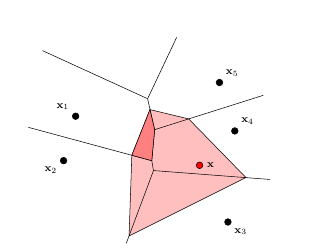
\includegraphics[width=0.6\linewidth]{slika6.png}
\caption*{\textsl{Slika 6. Najbliži susedi za tačku x}}
\end{figure}
Vrednost interpolacije u tački $x$ dobijamo tako što usrednjimo vrednosti ovih definisanih okolnih, susednih tačaka. 


 
\subsubsection{Barnes i Cressman interpolacija}
Barnes i Cressman spadaju u grupu sukcesivno korekcionih metoda, kod kojih se polje varijabli modifikuje koristeći osmotrene podatke iterativnim postupkom. Metod se zasniva na prolazu kroz svaku tačku mreže, ažuriranj varijabli za svaku od njih na osnovu osmotrenih podataka koje obuhvataju tu tačku mreže. Nakon prvog prolaza kroz zadato područje, radi se drugi prolaz, modifikujući polje svake tačke mrže u odnosu na okolne osmotrene tačke. Ove interacije se rade sve dok razlike između dve iteracije ne budu manje od zadatog praga.  
Polje mreže u tački $i$ se ažurira na sledeći način:
\begin{equation}
f_{i}^{m+1}=f_{i}^{m}+\frac{\sum_{k=1}^{K}w_{ik}^{m}(O_{k}-f_{k}^{m})}{\sum_{k=1}^{K}w_{ik}^{m}}
\end{equation}
gde $f_{i}^m$ je vrednost varijable u $i$-toj tački mreže za $m$ iteraciju. $O_k$ je vrednost $k$-te osmotrene vrednosti u okolini tačke mreže, a $w_{ik}^m$ je težinska funkcija i određuje se na sledeći način:
\begin{equation}
w_{ik}^m = exp(\frac{-r_{ik}^{2}}{2R_{m}^2})
\end{equation}
Za Cressman šemu težinska funkcija zavisi od radijusa delovanja $R_m$ kao:
\begin{equation}\label{key}
w_{ik}^m = \frac{R_{m}^{2}-r_{ik}^2}{R_{m}^{2}+r_{ik}^2}\quad za \quad r_{ik}^{2}\leq R_{m}^2
\end{equation}
\begin{equation}\label{key}
w_{ik}^{m}=0 \quad za \quad r_{ik}^{2}> R_{m}^2
\end{equation}
gde je $r_{ik}^2$ dužina između osmotrenih vrednosti i tačke mreže. Kod ove metode, osmotrene vrednosti izvan radijusa desejstva se ne uzimaju u ažuriranje vrednosti polja. 


\newpage


\section{Carpatclim aplikacija}

Na slici 7. je prikazan izgled aplikacije. Idući sa leve prema desnoj strani, u gornjem levom delu aplikacije mogućnosti koje aplikacija omogućava su sledeće: 
\begin{itemize}
	\item Yearly data (godišnje vrednosti temeperature) 
	\item Monthly data (mesečne vrednosti temperature)
	\item Daily data (dnevne vrednosti temperature)
	\item Points data (vrednosti tačke)
	\item Current weather (trenutno vreme)
\end{itemize}


\begin{figure}[h!]
	\centering
	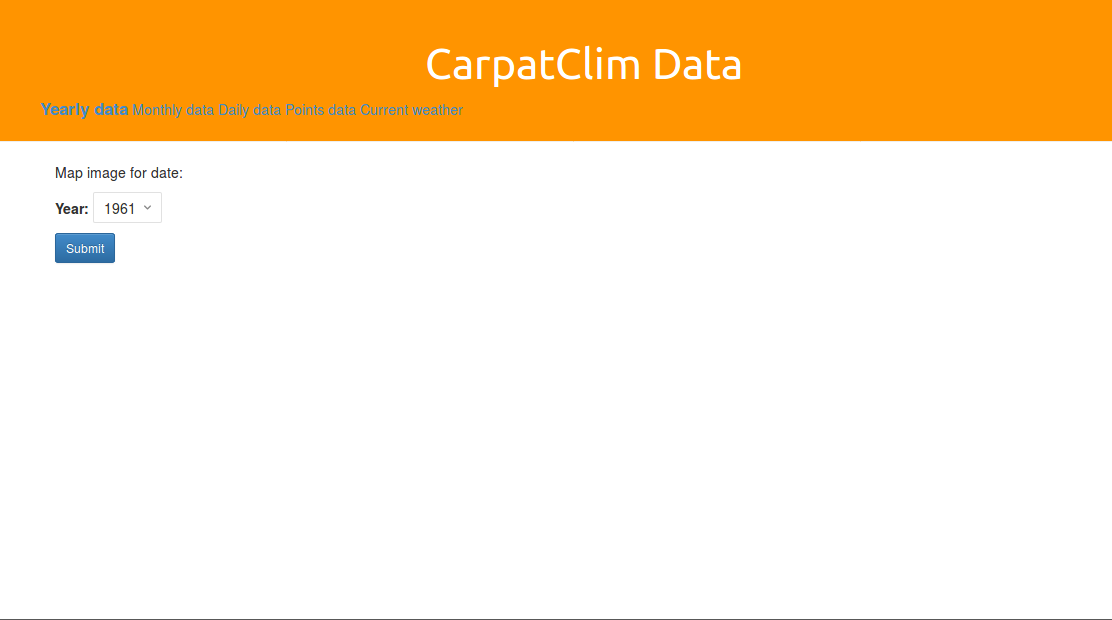
\includegraphics[width=1\linewidth]{aplikacija.png}
	\caption*{\textsl{Slika 7. Izgled aplikacije}}
\end{figure}

Prve tri opcije daju grafički prikaz srednjih temperatura za određeni interval, \textit{godišnje (yearl)} srednje temperature za izabranu godinu dok ostale dve opcije daju srednje vrednosti za \textit{mesečne (monthly)}, odnosno \textit{dnevne (daily)} vrednosti. \textit{Vrednosti tačke (Points data)} opcija daje informacije o izabranoj tački, izborom vrednosti longitude i latitude u mogućnosti smo videti u kojoj zemlji se nalazi tačka i na kojoj je visini. Opcija \textit{trenutno vreme (current weather)} daje trenutne vremenske podatke za izabrani grad. 


\subsection{Godišnje, mesečne, dnevne srednje vrednosti temperature}

Prilikom izbora jedo od ove tri opcije, pojavljuje se forma za izbor godine, meseca ili dana u zavisnosti da li želimo godišnje, dnevne ili mesečne vrednosti. Na slici 8. je prikazana forma za srednje dnevne vrednosti temperature.   



\begin{figure}[!htb]
\centering
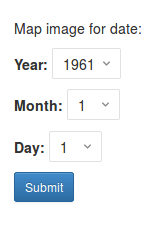
\includegraphics[width=0.2\linewidth]{Daily.png}
\caption*{\textsl{Slika 8. Forma za izbor godine, meseca, dana za prikaz srednje dnevne temperature}}
\end{figure}

Kao što sa slike 8. vidimo, postoji izbor za godinu koje se kreću u rasponu od 1961-2010, zatim izbor meseca i dana. Kada izaberemo željeni vremenski interval, aktiviranjem dugmeta \textit{submit} dobijamo grafički prikaz. 

\begin{figure}[!htb]
	\centering
	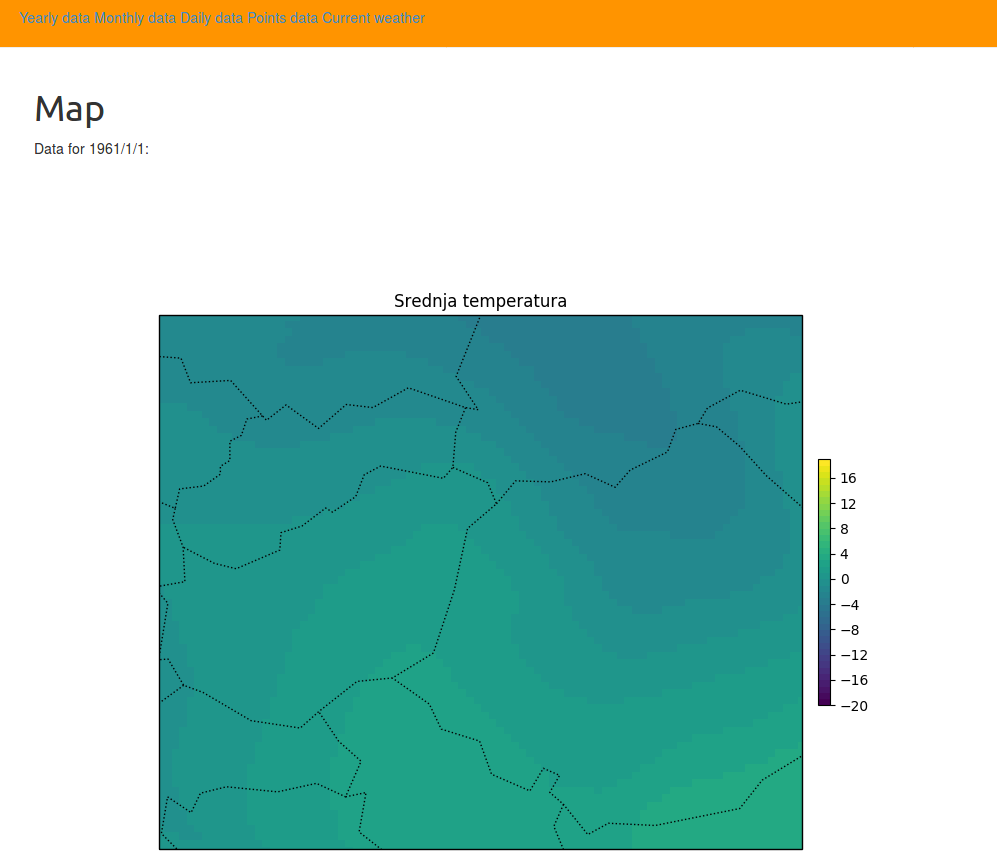
\includegraphics[width=0.6\linewidth]{mapa.png}
	\caption*{\textsl{Slika 9. Grafički prikaz polja srednje dnevne temperature za izabrani period 1961/1/1}}
\end{figure}

\subsection{Vrednosti tačke}
Sledeća opcija \textit{vrednost tačke(points data)} na daje opis tačke mreže za definisanu longitudu i latitudu. 

\begin{figure}[!htb]
	\centering
	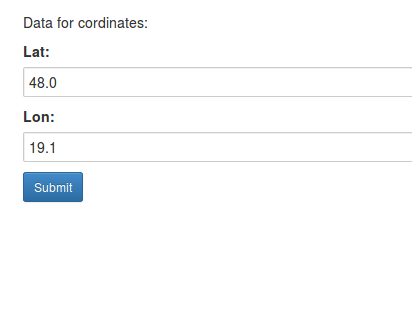
\includegraphics[width=0.7\linewidth]{points.png}
	\caption*{\textsl{Slika 10. Izbor latitude i longitude za tačku mreže}}
\end{figure}

Moguće vrednosti za latitudu su od 44-50 dok su za longitudu od 17-27. Izborom neke vrednosti za latitudu i longitudu dobijaju se podaci kao sa slike 11:

\begin{figure}[!htb]
	\centering
	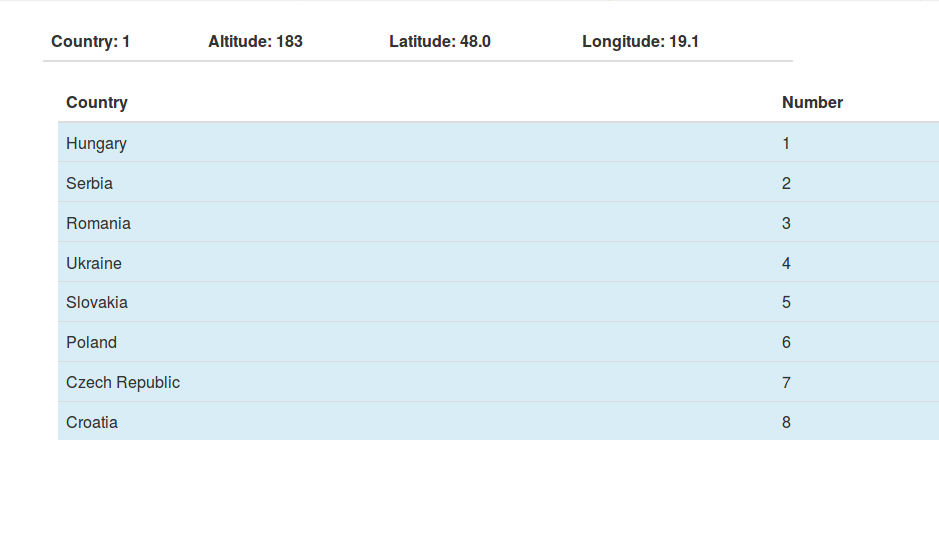
\includegraphics[width=0.7\linewidth]{data.png}
	\caption*{\textsl{Slika 11. Podaci za latidudu 48.0 i longitudu 19.1}}
\end{figure}
Sa slike 11. vidimo da se tačka sa datim kordinatam nalazi u Mađarskoj, i visina na kojoj su merene vrednosti meteoroloških promenljivih je 183.

\subsection{Trenutno vreme}
Ova aplikacija nam daje informacije o trenutinim vremenskim parametrima u izabranim gradovima. Kako bi izabrali željenu lokaciju, u polje "\textit{City Name}" upišemo ime grada.
\begin{figure}[!htb]
	\centering
	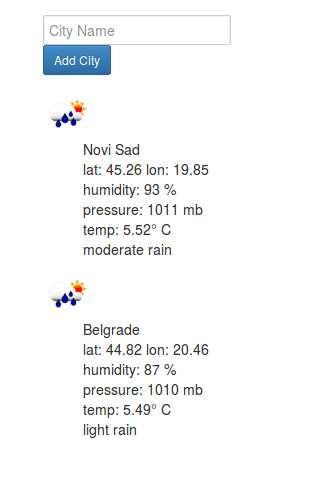
\includegraphics[width=0.5\linewidth]{vreme.png}
	\caption*{\textsl{Slika 12. Trenutni vremenski parametri u izabranim gradovima}}
\end{figure}


\end{document}
